\documentclass[11pt,aps,preprint,nofootinbib,superscriptaddress,tightenlines]{revtex4-2}
\usepackage{amsmath,amssymb,bm,mathtools}
\usepackage{graphicx}
\usepackage{xcolor}
\usepackage{tikz}
\definecolor{darkblue}{RGB}{0,0,160}
\usepackage{xr-hyper}
\usepackage[colorlinks=true,linkcolor=darkblue,citecolor=darkblue,urlcolor=darkblue]{hyperref}

\def\st{\begin{equation}}
\def\stp{\end{equation}}
\def\Teff{{\sf T}}
\def\Eq#1{eq.~(\ref{#1})}
\def\Sect#1{Sect.~\ref{#1}}
\def\Fig#1{Fig.~\ref{#1}}
\providecommand{\tr}{\operatorname{tr}}
\newcommand{\avg}[1]{\langle #1\rangle}
\usepackage{dsfont}
\newcommand{\one}{\mathds{1}}

\externaldocument[OL-]{bond_dissipation}
\newcommand{\EqOL}[1]{eq.~(\ref{OL-#1}) of Ref.~\cite{OneLevel}}
\newcommand{\SectOL}[1]{Sect.~\ref{OL-#1} of Ref.~\cite{OneLevel}}
\let\oldparagraph\paragraph
\renewcommand{\paragraph}{\par\medskip\oldparagraph}
\begin{document}

\title{Particle metrics: gradients and quadratic forms on general arrangements}
\author{D.~Teaney}
\affiliation{Department of Physics and Astronomy, Stony Brook University,
Stony Brook, New York 11794, USA}
\date{\today}

\begin{abstract}
On an irregular set of particles, gradients are obtained by fitting bond
differences, and quadratic forms in the gradients by bond sums.  Both are
controlled by the bond moment, the push-forward of the particles' own metric
to physical space.  The fit is exact for linear fields on any arrangement.
The bond sum is the physical quadratic form only if the bond moment is
proportional to the inverse metric of the fluid, flat at rest and comoving in
motion.  With bond weights evaluated at the comoving distance this holds for
smoothly distributed particles up to sampling corrections, which we measure
and remove with a small per-particle reweighting.
\end{abstract}

\maketitle


\section{Introduction and overview}
\label{sec:intro}

A particle method replaces a continuous fluid by a finite, irregular set of
points.  The continuum equations, however, are written in terms of gradients
of fields and of quadratic forms in those gradients, contracted with a
metric.  A dissipative function, for example, is the square of a strain rate.
On the particles both objects must be rebuilt from \emph{bonds}: the
separations $\bm r_{ab}$ between a particle and its neighbours, and the
differences $\Delta\phi_{ab}$ of the fields across them.  This note collects the
general machinery for doing so.  None of it is specific to dissipation, and it
applies to any arrangement of particles and to a moving fluid.

\paragraph{The idea.}  Two operations recur in any particle description.
\begin{enumerate}
\item \emph{Gradients} are obtained by fitting the bond differences of a field
  with a linear field (Operation 1).
\item \emph{Quadratic forms} in the gradients are obtained as weighted sums over
  bonds of products of differences (Operation 2).
\end{enumerate}
Both are controlled by a single matrix per particle, the \emph{bond moment}
$M_a$: the weighted second moment of the bond vectors of particle $a$.  It is
the matrix that is inverted to fit a gradient, and it is the metric that a bond
sum actually uses to contract two gradients.  The physics, on the other hand,
contracts gradients with the inverse metric of the fluid: the flat metric at
rest, and the comoving metric $\ell$ in motion.  The construction works when
these two agree.

\paragraph{The storyline.}  The note proceeds in the following steps.
\begin{itemize}
\item \Sect{sec:metric} introduces a general spatial metric $h_{ij}$, which
  covers both the fluid at rest and the moving fluid.  It measures bonds, through
  the comoving distance that sets the bond weights, and its inverse contracts
  gradients.
\item \Sect{sec:labels} defines the bond moment.  Labelling the particles by a
  reference lattice shows that the bond moment is the push-forward of the
  particles' own metric to physical space.  For smoothly distributed particles
  its continuum value is fixed by the metric in the weights.
\item Sections~\ref{sec:op1} and \ref{sec:op2} state the two operations.  The
  fit is exact for linear fields on any arrangement and needs only that $M_a$ be
  invertible.  The bond sum splits exactly into a resolved part, contracted with
  $M_a$, and a non-negative residual.  It is the physical quadratic form only if
  $M_a$ is proportional to the inverse metric.
\item \Sect{sec:weights} absorbs $n_a$ into normalized weights $w_{ab}$ and
  reads them as faces: the fit becomes Gauss's theorem and the bond sum a graph
  Laplacian.
\item \Sect{sec:sets} explains what sets $M_a$: the shape of the weights, not
  the arrangement of the particles.  The only departure is sampling error.
\item \Sect{sec:sampling} measures that sampling error, at rest and in motion.
\item \Sect{sec:Lambdacorr} removes it with a small per-particle reweighting
  $\Lambda_a$.  Sections~\ref{sec:limit} and \ref{sec:fail} show that $\Lambda_a$
  vanishes in the continuum limit and describe what the code does when it
  cannot be found.
\end{itemize}

\paragraph{Main results.}
\begin{itemize}
\item The fit, \Eq{Gfit}, is the chain rule through the particle map, and is
  exact on any arrangement and with any weights.
\item The bond sum obeys the exact identity \Eq{quadform}: resolved part plus
  residual.  For smooth fields the residual is smaller by $(h/L)^2$.
\item With weights evaluated at the comoving distance, the bond moment is
  proportional to the inverse metric up to sampling corrections,
  \Eq{Mapprox}.  The particles' arrangement, including a smooth deformation or
  a Lorentz contraction, does not enter.
\item The sampling error falls as $(a/h)^2$ for bounded disorder and grows by
  about $\gamma$ in motion.  The correction $\Lambda_a$, \Eq{Lambdadef}, removes it
  exactly.
\end{itemize}
Throughout, $d_s$ is the number of spatial dimensions spanned by the particles
($d_s=2$ in the figures).  In the application of Ref.~\cite{OneLevel} it need
not equal the physical dimension $d$ that appears in the bulk viscosity.

\paragraph{Notation.}  Particles sit at positions $\bm x_a$ and carry entropies
$s_a$.  The smoothed entropy density is $S(\bm x)=\sum_bs_bW(\bm x-\bm x_b)$, with an
SPH kernel $W$ of smoothing length $h$ and support $2h$.  Each particle is
assigned the volume its entropy occupies at the local entropy density,
\st
V_a=\frac{s_a}{S_a},\qquad S_a\equiv S(\bm x_a),
\label{Va}
\stp
which is the SPH quadrature weight, $\sum_aV_af(\bm x_a)\simeq\int f$.  Bonds
carry a weight $\psi_{ab}$ that is a function of the bond length, by default
$\psi=-W'/r$ with its own range $h_\psi$.  The typical particle spacing is $a$.
The fields $\phi$ are arbitrary.  In the application of Ref.~\cite{OneLevel},
where this machinery is used to build a one-level (bond) dissipative function,
the field is $\beta=\bm v/T$.

\section{The metric}
\label{sec:metric}

We first fix how bonds are measured and how gradients are contracted.  A
single metric does both, and choosing it is the only place where the motion of
the fluid enters.

All bond vectors $r^i_{ab}=x^i_b-x^i_a$ are taken at the same lab time.  We
measure them with a spatial metric $h_{ij}$ attached to particle $a$, and
contract gradients with its inverse $h^{ij}$, $h^{ij}h_{jk}=\delta^i{}_k$.  The two
cases are
\st
\begin{aligned}
&\text{at rest:} && h_{ij}=\delta_{ij}, && h^{ij}=\delta^{ij},\\
&\text{moving:} && h_{ij}=(\ell^{-1})_{ij}=\delta_{ij}+\gamma^2v_iv_j,\qquad && h^{ij}=\ell^{ij}=\delta^{ij}-v^iv^j .
\end{aligned}
\label{hmetric}
\stp
The metric always carries indices; a plain $h$ is the smoothing length.

\paragraph{Lengths.}  The length of a bond in the metric is the comoving distance
in the rest frame of $a$,
\st
\rho_{ab}^2=h_{ij}\,r^i_{ab}r^j_{ab}=\Delta_{\mu\nu}(u_a)\,\Delta x^\mu_{ab}\Delta x^\nu_{ab},
\qquad \Delta x^\mu_{ab}=(0,\bm r_{ab}) .
\stp
It is a Lorentz scalar, the distance between the two equal-lab-time points as
measured in the rest frame of $a$.  For a moving fluid $\det h_{ij}=\gamma^2$, so a
region of lab volume $\mathcal V$ has rest-frame volume $\gamma\mathcal V$.

\paragraph{Gradients.}  The inverse $h^{ij}$ is the metric that contracts spatial
gradients.  Consider a field that does not change along the flow,
\st
u^\mu\partial_\mu\phi=0,\qquad\text{i.e.}\qquad \partial_t\phi=-v^i\partial_i\phi .
\stp
Its rest-frame gradient squared is
\st
\Delta^{\mu\nu}\partial_\mu\phi\,\partial_\nu\phi
=g^{\mu\nu}\partial_\mu\phi\,\partial_\nu\phi+(u^\mu\partial_\mu\phi)^2
=\partial_i\phi\,\partial_i\phi-(v^i\partial_i\phi)^2
=h^{ij}\,\partial_i\phi\,\partial_j\phi .
\stp
This is how $\ell^{ij}$ enters the dissipative function of a moving fluid, as
$\tr(\ell S\ell S)$, and why the bond form must reproduce it.

\paragraph{Weights.}  The bond weights are evaluated at the comoving distance,
$\psi_{ab}=\psi(\rho_{ab})$.  They are round in the metric $h_{ij}$: the stencil
$\rho_{ab}<2h_\psi$ is a circle at rest and, for a moving fluid, an ellipse
contracted by $1/\gamma$ along $\bm v$.

\section{Labels and the bond moment}
\label{sec:labels}

With the metric in hand, we turn to the particles.  To see how their
arrangement enters, it helps to label them by a reference lattice and to
describe their positions as a map from labels to space.

Label each particle by the coordinates of a reference lattice, $a=\sigma^I$ with
$I=1,\dots,d_s$, for example the lattice the particles started on.  In this
reference configuration the positions coincide with the labels,
\st
x^i=\delta^i{}_I\,\sigma^I,\qquad r^i_{ab}=\delta^i{}_I\,\Delta\sigma^I_{ab}\qquad\text{(reference lattice)} .
\stp
As the fluid moves, the positions define a map $\bm x(\sigma)$, with deformation gradient
\st
e^i{}_I=\frac{\partial x^i}{\partial\sigma^I},\qquad
r^i_{ab}\simeq e^i{}_I\,\Delta\sigma^I_{ab} ,
\stp
and $e^i{}_I=\delta^i{}_I$ on the reference lattice.
Both operations are controlled by the bond moment
\st
M_a^{ij}=\sum_{b\neq a}V_b\,\psi_{ab}\,r^i_{ab}r^j_{ab} .
\label{Mdef}
\stp

\paragraph{The bond moment as a push-forward.}  The bond moment is the
translation between the particles and coordinate space.  The particles carry
their own (inverse) metric on the labels, the moment of the label differences,
\st
\mu^{IJ}=\sum_{b\neq a}V_b\,\psi_{ab}\,\Delta\sigma^I_{ab}\Delta\sigma^J_{ab} ,
\label{mudef}
\stp
with $\psi_{ab}=\psi(\rho_{ab})$ the physical weight as before.  The bond moment is
its push-forward by the particle map,
\st
M_a^{ij}=e^i{}_I\,\mu^{IJ}\,e^j{}_J ,
\label{pushforward}
\stp
and \Eq{Mtarget} below asks that it agree with $n_a h^{ij}$.  We never need to
evaluate $\mu^{IJ}$, which would require knowing each particle's place on the
reference lattice; it serves only to interpret $M_a$.

\paragraph{The continuum moment.}  Suppose the particles sample space
smoothly: finely on the scale of the stencil ($a\ll h$), and with volumes
$V_b=s_b/S_b$, \Eq{Va}, that compensate the local particle density.  The second
condition requires the density to vary slowly across the stencil ($h\ll L$),
since $S_b$ is smoothed over $h$.  The density itself need not be constant.  The
bond sum is then a quadrature of an integral,
\st
M_a^{ij}\simeq\int d^{d_s}r\;\psi(\rho)\,r^ir^j,\qquad \rho^2=h_{kl}r^kr^l .
\stp
The integral is evaluated by changing variables to the coordinates in which the
stencil is round, $s^i=(h^{1/2})^i{}_jr^j$, so that
\st
\rho=s\equiv|\bm s|,\qquad d^{d_s}r=\frac{d^{d_s}s}{\sqrt{\det h_{ij}}} .
\stp
By rotational symmetry in $\bm s$,
\st
\int d^{d_s}s\;\psi(s)\,s^ks^l=n_0\,\delta^{kl},
\stp
and so
\st
\int d^{d_s}r\;\psi(\rho)\,r^ir^j=\frac{n_0}{\sqrt{\det h_{ij}}}\;h^{ij},\qquad
n_0=\frac1{d_s}\int d^{d_s}s\;\psi(s)\,s^2 .
\label{Mcomoving}
\stp
Thus, for smoothly distributed particles,
\st
M_a^{ij}=n_a\,h^{ij}+\big(\text{sampling corrections}\big),\qquad n_a\simeq\frac{n_0}{\sqrt{\det h_{ij}}} .
\label{Mapprox}
\stp
The corrections are the sampling error of a finite, irregular star, which falls
with $h/a$, and an $O(h^2/L^2)$ error from the smoothed volumes.  They are
measured in \Sect{sec:sampling} and removed by $\Lambda_a$ in \Sect{sec:Lambdacorr}.
\Fig{fig:stencil2d} shows one star at rest and in motion.

\begin{figure}[t]
\centering
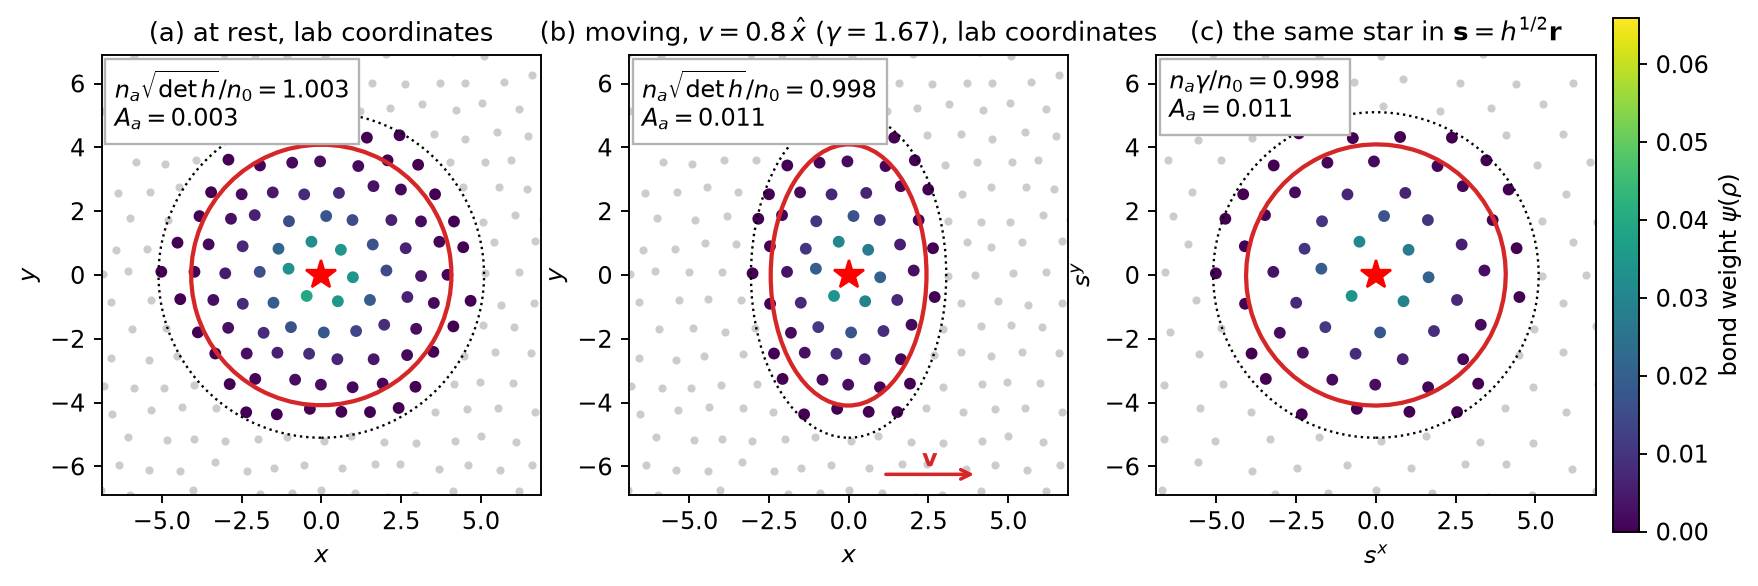
\includegraphics[width=\textwidth]{figs/stencil_metric.png}
\caption{One star (red star) on a jittered ($j=0.3$) hexagonal lab lattice,
$h/a=2.55$, $\psi=-W'/r$, and $V_b$ the lattice cell area.  Dots
inside the stencil $\rho<2h$ (dotted) are coloured by $\psi(\rho)$.  The red ellipse
is the measured moment, $\bm r^T(M_a/n_a)^{-1}\bm r=\text{const}$.
 (a)~At rest, $M_a\simeq n_0\one$.
 (b)~Moving with $v=0.8\,\hat x$ ($\gamma=5/3$): the stencil and the
moment are contracted along $\bm v$, and $M_a=(0.214,\,0.603)$ on the diagonal,
against $(n_0/\gamma)\ell=(0.216,\,0.600)$.
 (c)~The same star in $\bm s=h^{1/2}\bm r$, where
the stencil is round and the moment is isotropic, $n_a\gamma/n_0=0.998$.
 The residual anisotropy $A_a$ (\Sect{sec:sampling}) is the sampling error; it is
larger in motion because the contracted stencil holds $1/\gamma$ as many
neighbours.  Produced by \texttt{examples/stencil\_metric.py}.}
\label{fig:stencil2d}
\end{figure}

\section{Operation 1: gradients}
\label{sec:op1}

We now state the two operations.  The first rebuilds a gradient from bond
differences.  It uses the bond moment only through its inverse, and needs no
metric.

Let $\phi$ be any field carried by the particles: a component of $\beta$, a
temperature, a chemical potential, and so on.  Its bond differences are
\st
\Delta\phi_{ab}=\phi_b-\phi_a .
\stp
The gradient at $a$ is the linear field that best fits these differences:
\st
\nabla_i\phi=\arg\min_{g_i}\sum_{b\neq a}V_b\,\psi_{ab}\big(\Delta\phi_{ab}-g_j\,r^j_{ab}\big)^2 .
\stp
Setting the derivative with respect to $g_i$ to zero gives
\st
\nabla_i\phi=\tilde\nabla^j\phi\,(M_a^{-1})_{ji},\qquad
\tilde\nabla^j\phi=\sum_{b\neq a}V_b\,\psi_{ab}\,\Delta\phi_{ab}\,r^j_{ab} .
\label{Gfit}
\stp
Here $M_a^{ij}$ carries upper indices, so its inverse $(M_a^{-1})_{ij}$ carries lower ones.
Here $\nabla_i\phi$ always denotes this fit, a property of the particle; we write
$(\nabla_i\phi)_a$ when the particle must be explicit, and $\partial_i\phi$ for
the true derivative.  For the components of $\beta$, $\phi=\beta_k$, the fit
is the matrix $(\nabla\beta)_a$ with components $\nabla_i\beta_k$ of \EqOL{Gmin}.  The fit involves no metric: the
metric enters only through the weights.

Now suppose that $\phi$ is linear in the labels near $a$, so that
\st
\Delta\phi_{ab}=\frac{\partial\phi}{\partial\sigma^J}\,\Delta\sigma^J_{ab} .
\stp
With the label moment $\mu^{JK}$ of \Eq{mudef}, $\tilde\nabla^i\phi$ and the bond moment
become
\st
\tilde\nabla^i\phi=\frac{\partial\phi}{\partial\sigma^J}\,\mu^{JK}\,e^i{}_K,\qquad
M_a^{ij}=e^i{}_J\,\mu^{JK}\,e^j{}_K .
\stp
This gives the interpretation of $\tilde\nabla^i\phi$: it is the label gradient of $\phi$
with its index raised by $\mu^{JK}$ and pushed forward to physical space, i.e.\ the
gradient with its index raised by the bond moment, $\tilde\nabla^i\phi=M_a^{ij}\,\partial_j\phi$.
The fit lowers the index again with $M_a^{-1}$.  Inserting $\tilde\nabla^i\phi$ and
$M_a^{ij}$ into \Eq{Gfit}, the factors of $\mu$ cancel:
\st
\nabla_i\phi=\frac{\partial\phi}{\partial\sigma^J}\,(e^{-1})^J{}_i=\frac{\partial\phi}{\partial x^i} .
\stp
The fit is the chain rule through the particle map.  It is exact for any
arrangement, any weights and any metric, provided the full $M_a^{-1}$ is kept.

\section{Operation 2: quadratic forms}
\label{sec:op2}

The second operation is where the metric matters.  A quadratic form in two
gradients is built as a bond sum, and the question is which metric that sum
actually uses.

Let $\phi$ and $\chi$ be two fields, not necessarily linear.  Split each bond
difference into the part the fit captures and a residual:
\st
\Delta\phi_{ab}=\nabla_i\phi\,r^i_{ab}+\delta_{ab}(\phi),
\label{residual}
\stp
and similarly for $\chi$.  Because $\nabla_i\phi$ is the least-squares fit, the
residual is orthogonal to the bond vectors:
\st
\sum_{b\neq a}V_b\,\psi_{ab}\,\delta_{ab}(\phi)\,r^j_{ab}=\tilde\nabla^j\phi-\nabla_i\phi\,M_a^{ij}=0 .
\label{orthog}
\stp
When the bond sum of the products of differences is expanded, the cross terms
therefore vanish.  This leaves the exact identity
\st
\sum_{b\neq a}V_b\,\psi_{ab}\,\Delta\phi_{ab}\,\Delta\chi_{ab}
=\nabla_i\phi\;M_a^{ij}\;\nabla_j\chi
+\sum_{b\neq a}V_b\,\psi_{ab}\,\delta_{ab}(\phi)\,\delta_{ab}(\chi) .
\label{quadform}
\stp
It holds for any arrangement, any weights and any fields.  For $\phi=\chi$ the
residual term is non-negative.  The first term is the \emph{resolved} part and
the second the \emph{residual}.  Three remarks on the size of the residual:
\begin{itemize}
\item \emph{Smooth fields.}  For a field that varies on a scale $L\gg h$, the
  residual is the curvature of the field across the star,
  \st
  \delta_{ab}(\phi)\simeq\tfrac12\,\partial_i\partial_j\phi\;r^i_{ab}r^j_{ab}
  -\big(\text{its fitted linear part}\big) .
  \stp
  The residual term in \Eq{quadform} is then smaller than the resolved term by
  a factor of order $h^2/L^2$.  Because the cross terms vanish exactly,
  the correction is second order in the curvature, not first.
\item \emph{Fit versus true gradient.}  The identity is written in terms of the
  fit $\nabla_i\phi$, so it contains no error from the fit itself.  The fit
  differs from the true $\partial_i\phi$ by $O(h^2\,\partial^3\phi)$ on a
  symmetric star and by $O(h\,\partial^2\phi)$ on an irregular one.  For an exactly
  linear field the residual vanishes and the fit is the true gradient, so the
  identity holds with no correction.
\item \emph{Unresolved modes.}  For wavelengths comparable to the
  particle spacing, such as the zigzag mode, the fit captures little and the
  residual is not small.  It is the residual that damps these modes, see
  \EqOL{split2d}.
\end{itemize}
The resolved term contracts the two gradient indices with $M_a$.  The physics
wants them contracted with $h^{ij}$.  The resolved part is therefore the
physical quadratic form only if
\st
M_a^{ij}=n_a\,h^{ij} ,
\label{Mtarget}
\stp
that is $M_a=n_a\one$ at rest and $M_a=n_a\ell_a$ for a moving fluid.  For a
vector field such as $\beta$, each pair of components $\beta^k,\beta^l$ enters
\Eq{quadform}, and the component indices are contracted separately, again with
$h_{kl}$ or $h^{kl}$ as their position requires.

\section{Normalized weights: faces, Gauss and the Laplacian}
\label{sec:weights}

When the target \Eq{Mtarget} holds, the factor $n_a$ can be absorbed into the
weights.  The resulting normalized weights have a simple geometric meaning, and
they connect the bond construction to finite volumes and to graph Laplacians.

Define
\st
w_{ab}=\frac{V_b\,\psi_{ab}}{n_a},\qquad
\sum_{b\neq a}w_{ab}\,r^i_{ab}r^j_{ab}=h^{ij} .
\label{wdef}
\stp
The second equation is \Eq{Mtarget}.  The weights have units of
$1/\text{length}^2$, and they belong to particle $a$: $w_{ab}\neq w_{ba}$ in
general.  We use $V_b\psi_{ab}$ in Operations 1 and 2, where $M_a$ is
arbitrary, and $w_{ab}$ once \Eq{Mtarget} is imposed (with the corrected weights
of \Sect{sec:Lambdacorr} it holds exactly).

\paragraph{Faces.}  Define the face vector of the bond,
\st
A^i_{ab}=V_a\,w_{ab}\,r^i_{ab},\qquad
\sum_{b\neq a}A^i_{ab}\,r^j_{ab}=V_a\,h^{ij} .
\label{Adef}
\stp
$A^i_{ab}$ has units of area and points along the bond.  Its normal covector,
\st
A_{ab\,i}=h_{ij}\,A^j_{ab},\qquad \sum_{b\neq a}A_{ab\,i}\,r^j_{ab}=V_a\,\delta_i{}^j ,
\stp
makes the face orthogonal to the bond in the metric $h$, i.e.\ in the rest frame
of $a$.  Then
\st
V_a\,w_{ab}=\frac{|\bm A_{ab}|}{|\bm r_{ab}|},
\stp
the face area over the distance between the particles.  In finite volumes this
ratio is the transmissibility of the face.  The closure is the discrete form of
$\oint x^j\,d\Sigma_i=V\delta_i{}^j$, with the factor of two from pairing the face
with the full bond rather than the half-bond to its centre absorbed into
$A_{ab}$.  A momentum flux $\Pi^{ij}$ at $a$ gives the momentum $\Pi^{ij}A_{ab\,j}$
to $b$ through the face.  This quantity (known as the traction) is the momentum
given by $a$ to $b$ along the bond $ab$.\footnote{In much of the literature on
elasticity the traction is minus this quantity.}  The closure recovers the flux from its faces,
\st
\sum_{b\neq a}\Pi^{ik}A_{ab\,k}\,r^j_{ab}=V_a\,\Pi^{ij} .
\stp

\paragraph{Gauss.}  With \Eq{wdef} the fit \Eq{Gfit} becomes
\st
\nabla_i\phi=h_{ij}\sum_{b\neq a}w_{ab}\,\Delta\phi_{ab}\,r^j_{ab}
=\frac{1}{V_a}\sum_{b\neq a}\Delta\phi_{ab}\,A_{ab\,i} .
\label{Ggauss}
\stp
This is the finite-volume gradient: the flux of $\phi$ through the faces divided
by the volume.  It is written with differences, and the closure makes it exact for
linear fields.  The moment-weighted gradient is now $\tilde\nabla^i\phi=n_a\,h^{ij}\nabla_j\phi$.

\paragraph{Graph Laplacian.}  For a smooth field on a symmetric star the first
moment $\sum_bw_{ab}r^i_{ab}$ vanishes, and expanding
$\Delta\phi_{ab}=r^i\partial_i\phi+\frac12r^ir^j\partial_i\partial_j\phi$ gives
\st
\sum_{b\neq a}w_{ab}\,(\phi_b-\phi_a)\simeq\frac12\,h^{ij}\partial_i\partial_j\phi .
\label{graphlap}
\stp
So $2w_{ab}$ are the edge weights of a consistently normalized graph Laplacian,
in the metric $h$.  Its quadratic form is the bond sum of Operation 2,
\st
E[\phi]=\frac12\sum_aV_a\sum_{b\neq a}w_{ab}\,(\Delta\phi_{ab})^2
=\frac12\sum_aV_a\big[h^{ij}\nabla_i\phi\,\nabla_j\phi+\text{residual}\big]
\;\longrightarrow\;\frac12\int h^{ij}\,\partial_i\phi\,\partial_j\phi ,
\stp
by \Eq{quadform}.  Its derivative is a sum over bonds with the symmetric
weights $c_{ab}=V_aw_{ab}+V_bw_{ba}$,
\st
-\frac{\partial E}{\partial\phi_a}=\sum_{b\neq a}c_{ab}\,(\phi_b-\phi_a)
\simeq V_a\,h^{ij}\partial_i\partial_j\phi ,
\stp
the graph Laplacian on the bonds.  It has $\phi=$ const as its only zero mode
when the bonds connect all particles, and every bond contributes a non-negative
amount to $E$.

\paragraph{On a grid.}  For nearest neighbours at spacing $\Delta x$ at rest,
\Eq{wdef} gives $w_{ab}=1/(2\Delta x^2)$, so $V_aw_{ab}=\Delta x^{d_s-1}/(2\Delta x)$,
half the face area over the spacing.  The bond Laplacian is then
$\sum_bc_{ab}(\phi_b-\phi_a)=V_a\sum_b(\phi_b-\phi_a)/\Delta x^2$, the standard
finite-difference Laplacian times the cell volume.

\section{What sets the bond moment}
\label{sec:sets}

Operation 2 requires the bond moment to equal the inverse metric, up to
normalization.  Here we collect what determines the bond moment, and so whether
the requirement can hold.

\paragraph{The shape of the weights.}  Weights that are round in a metric give a
moment proportional to the inverse of that metric, \Eq{Mcomoving}.  This is why
$\psi$ is evaluated at the comoving distance: it makes the continuum moment
satisfy \Eq{Mtarget}, with $n_a\simeq n_0/\sqrt{\det h_{ij}}$.

\paragraph{The arrangement does not enter.}  The weights must be attached to
physical (comoving) distances.  For contrast, consider
\emph{reference-lattice weights}: each bond keeps the weight it had on the
reference lattice, $\psi(|\Delta\sigma_{ab}|)$, which is never updated as the
particles move, as on a mesh.  Then $\mu^{JK}=\mu_0\delta^{JK}$ is fixed, and
\st
M_a^{ij}=\mu_0\,e^i{}_J\,e^j{}_J ,
\stp
the inverse of the metric $e^i{}_Ie^i{}_J$ that the deformation induces on the
reference lattice.  The moment would record the deformation.  With physical weights a smoothly deformed lattice is still a
uniform point set, and the deformation drops out of $M_a$.  This includes the
Lorentz contraction: a lattice uniform in the fluid rest frame is a contracted
lattice in the lab, and the weights $\psi(\rho)$ still give $M_a\propto h^{ij}$.  The
metric in the weights sets the moment; the arrangement does not.

\paragraph{The sampling.}  A finite, irregular set of neighbours gives $M_a$ a
sampling error.  With physical weights the sampling error is the only source of
anisotropy.  It is removed by the correction $\Lambda_a$ below.

So the fit never needs \Eq{Mtarget}, while the quadratic form does.  The
mean-field form of \SectOL{sec:mf2d} uses both operations.  Operation 1 gives
$\Omega_a$ and $\theta_a$.  The covariant bond differences $\mathcal D_{ab}\beta$ of \EqOL{Dab} then
enter the quadratic form of Operation 2.  If \Eq{Mtarget} fails, directions that
happen to be over-represented among the neighbours are over-weighted in
$K$ of \EqOL{KMF}.

\section{The sampling error}
\label{sec:sampling}

The previous section left sampling error as the only departure from the
target.  We now measure its size, first at rest and then in motion.  The
measure is the anisotropy of the moment relative to its target,
\st
A_a=\frac{\big|\hat M_a-\frac1{d_s}\tr\hat M_a\,\one\big|}{\frac1{d_s}\tr\hat M_a},
\qquad \hat M_a=h^{1/2}M_ah^{1/2} ,
\stp
which vanishes exactly when \Eq{Mtarget} holds.  \texttt{examples/moment\_sampling.jl}
measures it at rest for a perfect hexagonal lattice, jittered lattices (each
particle shifted uniformly in $\pm ja/2$ per coordinate, the convention of
\texttt{setup\_ic}), random (Poisson) particles, and a lattice under a smooth
10\% shear, with physical and, for contrast, reference-lattice weights (\Fig{fig:moment},
Table~\ref{tab:moment}).
\begin{itemize}
\item The perfect lattice gives $A_a=0$.  The smooth shear gives $A_a\sim10^{-4}$
  with physical weights, falling rapidly with $h/a$; with reference-lattice weights it gives
  $A_a=0.26$ at every resolution.
\item Jitter gives a genuine sampling error, linear in the amplitude and falling
  as $(a/h)^2$:
  \st
  \overline{A}_a\simeq0.4\,j\,\Big(\frac{a}{h}\Big)^2 ,
  \label{Ascaling}
  \stp
  with the maximum about three times the mean.  Each of the
  $N_{\rm nb}\sim(h/a)^2$ neighbours shifts the moment by a random relative amount
  $\sim(ja/h)/N_{\rm nb}$; in quadrature these give $\sim j(a/h)^2$.
\item Poisson particles converge only as $1/\sqrt{N_{\rm nb}}\sim a/h$, since each
  neighbour contributes an $O(1)$ random amount.  At $h/a=2.55$ the mean is $0.17$
  and the maximum $0.54$.  Poisson-like disorder is where $\Lambda_a$ is most likely
  to fail.
\end{itemize}

\paragraph{Moving fluid.}  For a moving fluid the stencil $\rho<2h_\psi$ covers
a lab area smaller by $1/\gamma$, so it holds $1/\gamma$ as many neighbours, and the
sampling error grows accordingly.  For a jittered ($j=0.3$) lab lattice, with
1000 random stars per entry and $A_a$ computed with $\hat M_a$:
\begin{center}
\begin{tabular}{c c | c c c | c c c}
\hline\hline
 & & \multicolumn{3}{c|}{$h/a=2.55$} & \multicolumn{3}{c}{$h/a=4$}\\
$\bm v$ & $\gamma$ & $N_{\rm nb}$ & mean & max & $N_{\rm nb}$ & mean & max\\
\hline
$0$               & 1     & 91 & $1.8\times10^{-2}$ & $5.1\times10^{-2}$ & 233 & $7.3\times10^{-3}$ & $2.3\times10^{-2}$\\
$0.5\,\hat x$     & 1.155 & 81 & $2.1\times10^{-2}$ & $7.0\times10^{-2}$ & 203 & $8.7\times10^{-3}$ & $2.8\times10^{-2}$\\
$0.8\,\hat x$     & 1.667 & 57 & $3.2\times10^{-2}$ & $9.2\times10^{-2}$ & 138 & $1.30\times10^{-2}$ & $3.8\times10^{-2}$\\
$0.8\,(\hat x+\hat y)/\sqrt2$ & 1.667 & 54 & $3.2\times10^{-2}$ & $1.0\times10^{-1}$ & 137 & $1.32\times10^{-2}$ & $3.8\times10^{-2}$\\
\hline\hline
\end{tabular}
\end{center}
The direction of $\bm v$ relative to the lattice does not matter, and the mean
grows roughly as $\gamma$ (by $1.78$ at $\gamma=1.67$).  \Eq{Ascaling} becomes
\st
\overline{A}_a\simeq0.4\,j\,\gamma\,\Big(\frac{a}{h}\Big)^2 .
\stp
The effective resolution is set by
the rest-frame spacing, not the lab spacing.

\begin{figure}[t]
\centering
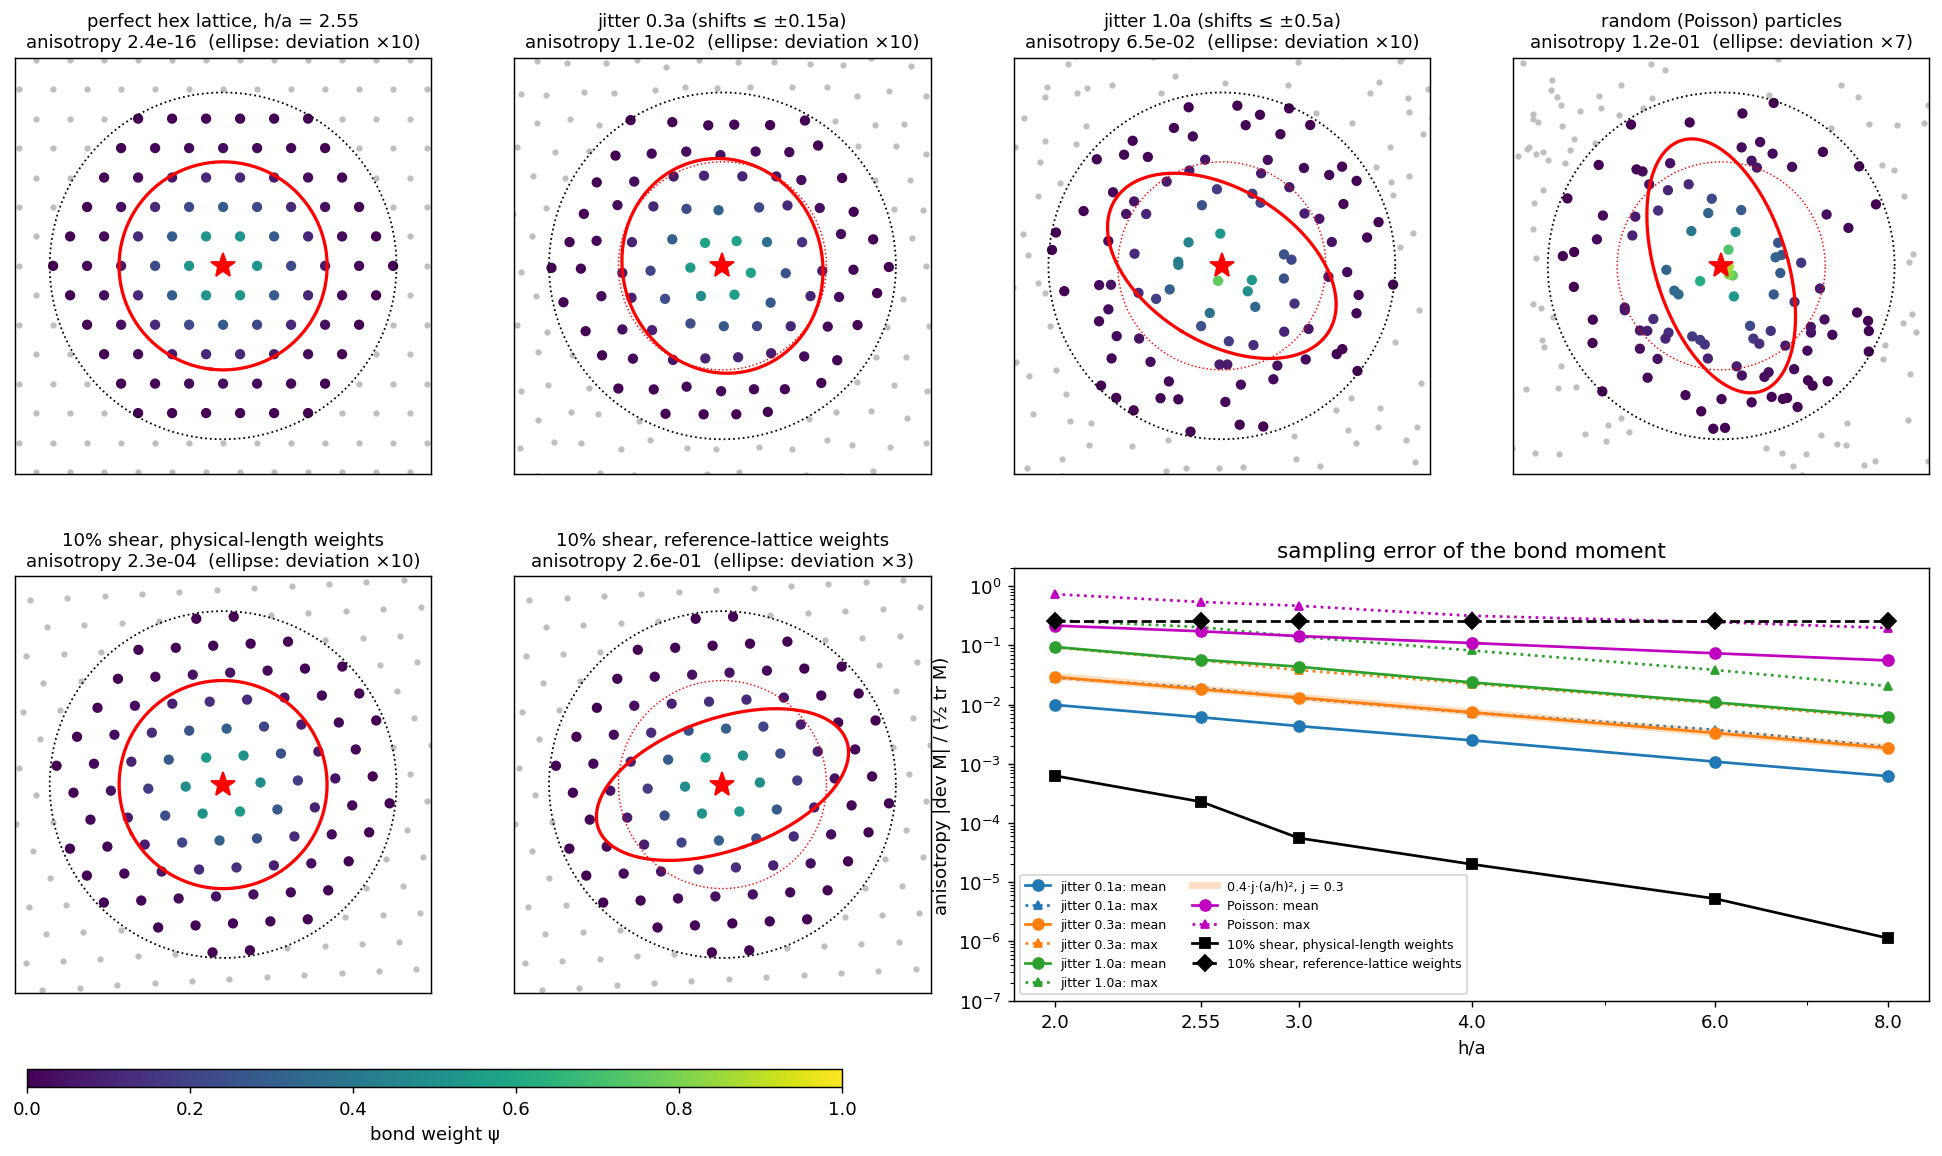
\includegraphics[width=\textwidth]{figs/moment_sampling.png}
\caption{The bond moment as a sampled quantity.  Six star panels: the star of
the particle marked by the red star at $h/a=2.55$ (dots coloured by the bond
weight $\psi$, kernel support dotted).  The red ellipse is the normalized moment
$M_a/(\frac12\tr M_a)$, with its deviation from the unit circle (red dotted)
exaggerated by the factor shown.  Bottom right: mean (circles) and maximum
(triangles) anisotropy over 2000 random stars as a function of $h/a$.  The
curves are for jitters $0.1a$, $0.3a$, $1.0a$ (shifts uniform in $\pm ja/2$) and for
Poisson particles, together with the smooth 10\% shear for physical-length
(black squares, the code) and reference-lattice (black diamonds, mesh-like:
each bond keeps its weight from the undeformed lattice) weights.  The shaded line
is \Eq{Ascaling} for $j=0.3$.}
\label{fig:moment}
\end{figure}

\begin{table}[t]
\centering
\begin{tabular}{c c | c c | c c | c c | c c | c c}
\hline\hline
 & & \multicolumn{2}{c|}{jitter $0.1a$} & \multicolumn{2}{c|}{jitter $0.3a$} &
 \multicolumn{2}{c|}{jitter $1.0a$} & \multicolumn{2}{c|}{Poisson} & \multicolumn{2}{c}{10\% shear}\\
$h/a$ & $N_{\rm nb}$ & mean & max & mean & max & mean & max & mean & max & phys. & ref.\\
\hline
2.00 & 58  & 9.9e-3 & 2.9e-2 & 2.9e-2 & 9.3e-2 & 9.4e-2 & 0.27 & 0.22 & 0.73 & 6.3e-4 & 0.26\\
2.55 & 90  & 6.1e-3 & 1.9e-2 & 1.8e-2 & 5.6e-2 & 5.7e-2 & 0.20 & 0.17 & 0.54 & 2.3e-4 & 0.26\\
3.00 & 124 & 4.3e-3 & 1.3e-2 & 1.3e-2 & 3.8e-2 & 4.4e-2 & 0.14 & 0.14 & 0.47 & 5.6e-5 & 0.26\\
4.00 & 238 & 2.5e-3 & 7.3e-3 & 7.4e-3 & 2.3e-2 & 2.4e-2 & 8.2e-2 & 0.11 & 0.32 & 2.0e-5 & 0.26\\
6.00 & 514 & 1.1e-3 & 3.8e-3 & 3.3e-3 & 1.0e-2 & 1.1e-2 & 3.9e-2 & 7.4e-2 & 0.25 & 5.3e-6 & 0.26\\
8.00 & 928 & 6.2e-4 & 1.9e-3 & 1.9e-3 & 5.9e-3 & 6.2e-3 & 2.1e-2 & 5.6e-2 & 0.20 & 1.1e-6 & 0.26\\
\hline\hline
\end{tabular}
\caption{Anisotropy $A_a$ of the bond moment (2000 random stars per entry).
$N_{\rm nb}$ is the number of neighbours inside the support $2h$ on the
lattice.  Jitter $j$: shifts uniform in $\pm ja/2$ per coordinate.  Shear:
physical-length weights (phys., the code) and reference-lattice weights (ref.).  Between
$h/a=2.55$ and 8 the means fall as $(h/a)^{-2.00}$ (jitter $0.3a$),
$(h/a)^{-1.94}$ (jitter $1.0a$) and $(h/a)^{-0.99}$ (Poisson).}
\label{tab:moment}
\end{table}

\section{Sampling corrections: $\Lambda_a$}
\label{sec:Lambdacorr}

The sampling error is small but not negligible at the resolutions used in
practice.  Rather than accept it, we remove it particle by particle with a small
change of the bond weights.

We reweight the bonds of each particle so that \Eq{Mtarget} holds exactly.  The
corrected weight is
\st
\psi_{ab}\;\to\;\psi_{ab}\big(1+\Lambda_{a,kl}\,r^k_{ab}r^l_{ab}\big),
\stp
with $\Lambda_{a,kl}$ symmetric and carrying lower indices.  Together with the
number $n_a$, it is defined by
\st
\boxed{\;
\sum_{b\neq a}V_b\,\psi_{ab}\big(1+\Lambda_{a,kl}\,r^k_{ab}r^l_{ab}\big)\,r^i_{ab}r^j_{ab}=n_a\,h^{ij},
\qquad h^{kl}\Lambda_{a,kl}=0 .\;}
\label{Lambdadef}
\stp
The first relation is $d_s(d_s+1)/2$ equations, one for each component of a
symmetric matrix; the second is one more.  Together they form a linear system
for the $d_s(d_s+1)/2$ components of $\Lambda_a$ and $n_a$.  The trace condition fixes
the remaining freedom: a part $\Lambda_{a,kl}\propto h_{kl}$ would multiply each
weight by $1+c\rho^2$, changing the radial profile of $\psi$ rather than the shape
of the moment, and only rescaling $n_a$.  Taking the $h$-trace of the first
relation gives
\st
n_a=\frac1{d_s}\sum_{b\neq a}V_b\,\psi_{ab}\big(1+\Lambda_{a,kl}\,r^k_{ab}r^l_{ab}\big)\,\rho_{ab}^2 .
\stp

\paragraph{Relation to inverting $M_a$.}  To first order in the anisotropy, work
in the coordinates $\bm s=h^{1/2}\bm r$, where the target is $\one$.  The fourth moment of
an isotropic star is
\st
\sum_bc_b\,s_is_js_ks_l=\frac{\mu_4}{d_s(d_s+2)}\big(\delta_{ij}\delta_{kl}+\delta_{ik}\delta_{jl}+\delta_{il}\delta_{jk}\big),
\qquad c_b=V_b\psi_{ab},\quad \mu_4=\sum_bc_b\,\rho_{ab}^4 .
\stp
Transforming back,
\st
\Lambda_{a,ij}\simeq-\frac{d_s(d_s+2)}{2\mu_4}\Big(h_{ik}M_a^{kl}h_{lj}-\frac1{d_s}\big(h_{kl}M_a^{kl}\big)\,h_{ij}\Big).
\label{Lambdalin}
\stp
At rest in two dimensions the prefactor is $4/\mu_4$.  Bonds along
over-represented directions are down-weighted in proportion to the deviator of
$M_a$ relative to $h^{ij}$.  The reweighting is the weight-space version of
acting on the moment with $n_a\,h^{il}(M_a^{-1})_{lk}$: it removes the shape of $M_a$
and leaves its size to $n_a$.

\paragraph{At rest in two dimensions.}  Write $\bm r_{ab}=(x,y)$.  A traceless
$\Lambda_a$ has two components,
\st
\bm r^T\Lambda_a\bm r=\Lambda_a^{xx}(x^2-y^2)+2\Lambda_a^{xy}xy ,
\stp
and the conditions $M_a^{xx}=M_a^{yy}$ and $M_a^{xy}=0$ are linear in them:
\st
\begin{pmatrix}
\sum_bc_b(x^2-y^2)^2 & 2\sum_bc_b\,xy(x^2-y^2)\\[2pt]
\sum_bc_b\,xy(x^2-y^2) & 2\sum_bc_b\,x^2y^2
\end{pmatrix}
\begin{pmatrix}\Lambda_a^{xx}\\ \Lambda_a^{xy}\end{pmatrix}
=-\begin{pmatrix}\sum_bc_b(x^2-y^2)\\ \sum_bc_b\,xy\end{pmatrix},
\label{Lambdasolve}
\stp
with $n_a$ then given by the trace.  The right-hand side is the
sampling anisotropy, so $\Lambda_a=0$ on the perfect lattice; \Eq{Lambdalin} agrees
with the exact solution to a few percent on jittered stars at $h/a=2.55$.

\paragraph{Moving fluid.}  Here $h^{ij}=\ell_a^{ij}$ and the weights are
$\psi(\rho_{ab})$ with $\rho_{ab}^2=r^T\ell_a^{-1}r$.  Equation \eqref{Lambdadef}
then reads
\st
\sum_{b\neq a}V_b\,\psi(\rho_{ab})\big(1+\bm r_{ab}^T\Lambda_a\bm r_{ab}\big)\,\bm r_{ab}\bm r_{ab}^T=n_a\,\ell_a,
\qquad \ell_a^{kl}\Lambda_{a,kl}=0 .
\stp
In 2D this is a $4\times4$ linear system for the three components of the symmetric
$\Lambda_a$, constrained by the trace condition, and $n_a$.  At rest $\Lambda_a$ also had
three components, but there we enforced the trace condition
$\Lambda_a^{xx}+\Lambda_a^{yy}=0$ directly.  The $4\times4$ system is what the code solves
(\texttt{bond\_weights\_comoving} in \texttt{src/celllist.jl}; the at-rest case
is the same routine with $\ell_a=\one$).  Three points:
\begin{itemize}
\item Each ingredient has a role.  $\psi(\rho)$ makes the continuum moment
  comoving, \Eq{Mcomoving}.  $\Lambda_a$ only removes the sampling error, and it is
  traceless with respect to $\ell_a$, not $\one$.  Without $\psi(\rho)$, $\Lambda_a$ would
  have to absorb the $O(v^2)$ anisotropy $\ell_a-\one$ itself, which does not vanish
  as $h/a\to\infty$.
\item The normalization is $n_a\simeq n_0/\gamma_a$, with corrections of the size
  of the sampling error.
\item In one dimension the moment is a number, a traceless $\Lambda_a$ vanishes,
  and no correction is needed; the moment itself fixes $n_a$.
\end{itemize}

The corrected weights are used everywhere: in the fit, in $K$ of \EqOL{KMF}, and in
$n_a$.

\section{The limit $h/a\to\infty$}
\label{sec:limit}

The correction $\Lambda_a$ is a discretization device, and it should disappear
in the continuum.  We check that it does.

What enters the weights is the dimensionless $\bm r^T\Lambda_a\bm r$ with $\rho<2h$,
and by \Eq{Lambdalin} it is of the order of the anisotropy $A_a$.  Hence
\st
\big|\bm r^T\Lambda_a\bm r\big|\;\lesssim\;O\Big(j\,\gamma\,\frac{a^2}{h^2}\Big)+O\Big(\frac{h^2}{L^2}\Big)\;\longrightarrow\;0
\qquad(a\ll h\ll L).
\label{Lambdalimit}
\stp
The first term is the sampling error \Eq{Ascaling} for disorder bounded at the
particle scale; for Poisson-like disorder it is replaced by $O(a/h)$.  The second term comes
from an anisotropic curvature of the density on a scale $L$ (the volume weights
$V_b=s_b/S_b$ compensate the density itself, and a linear gradient cancels by
symmetry).  So $\Lambda_a$ is a pure discretization correction, like a kernel
renormalization, and disappears in the continuum.  The exception is a boundary,
where the star is one-sided and $M_a$ is anisotropic at $O(1)$; in the periodic
box there are no boundaries.

\section{When the reweighting fails}
\label{sec:fail}

Finally, the linear system for $\Lambda_a$ can produce negative weights when a
neighbourhood is very poorly sampled.

If the neighbourhood is sampled too poorly, a corrected weight
$1+\bm r^T\Lambda_a\bm r$ can turn negative.  The code then falls back to
$\Lambda_a=0$, with $n_a$ from the trace of the uncorrected moment.  The fit remains exact, but for
that particle the resolved part of \Eq{quadform} is $\nabla_i\phi\,M_a^{ij}\,\nabla_j\phi$ rather than
the physical $n_a\,h^{ij}\,\nabla_i\phi\,\nabla_j\phi$.


\section{Summary}

Gradients and quadratic forms on particles are both governed by the bond
moment, the push-forward of the particles' metric to physical space.  The fit
of a gradient is exact on any arrangement.  The bond sum is the physical
quadratic form when the bond moment equals the inverse metric of the fluid.  Bond
weights evaluated at the comoving distance achieve this for smoothly
distributed particles, at rest and in motion, up to a sampling error that falls
as $(a/h)^2$ for bounded disorder.  The per-particle correction $\Lambda_a$ removes
that error exactly and vanishes in the continuum limit.

\begin{thebibliography}{9}
\bibitem{OneLevel} D.~Teaney, ``One-level (bond) dissipation on particles: one
and two dimensions, at rest and in motion'', notes (\texttt{bond\_dissipation.tex}).
\end{thebibliography}

\end{document}
